\documentclass[11pt,oneside]{amsart}
\usepackage{geometry}
\usepackage{amssymb,parskip,mathtools,microtype,pgfplots}
\usepackage[shortlabels]{enumitem}
\usepackage[most]{tcolorbox}

\usepgfplotslibrary{fillbetween,decorations.softclip}
\pgfplotsset{compat=1.18}

\definecolor{sol}{rgb}{0.1, 0.3, 0.6}

\newtcolorbox{solution}{enhanced, breakable, colframe=sol, title=Solution}

\theoremstyle{definition}
\newtheorem{problem}{Problem}

\newcommand{\bC}{\mathbb{C}}
\newcommand{\bQ}{\mathbb{Q}}
\newcommand{\bR}{\mathbb{R}}
\newcommand{\bZ}{\mathbb{Z}}

\title{MATH1103 Fall 2022\\
Problem Set 3}

\begin{document}
    \maketitle
    This problem set is due on Wednesday, September 21 at 11:59 pm. Each problem part is worth 3 points. Collaboration is encouraged. In all cases, you must write your own solutions, and and you must cite collaborators and resources used.

    \begin{problem}
        Some exercises.
        \begin{enumerate}[(a)]
            \item (Strang 5.4.1) Find
            \[\int\sqrt{2+x}\,dx.\]
            (Don't forget to add $+C$ to your final answer.)
            \begin{solution}
                We make the $u$-substitution $u=2+x$ and $du=dx$, to get $\int\sqrt{2+x}\,dx=\int u^{1/2}\,du=\frac 23 u^{\frac32}+C=\frac 23 (2+x)^{\frac32}+C$.
            \end{solution}
            \item (Strang 5.4.14) Find
            \[\int t^3\sqrt{1-t^2}\,dt.\]
            \emph{Hint}: Starting with $u=1-t^2$ worked for me.
            \begin{solution}
                We make the $u$-substitution $u=1-t^2$, $du=-2t\,dt$. The trick is to split up $t^3$ into $t^2\cdot t$ and then use $t^2=1-u$ to write $t^3\sqrt{1-t^2}$ as $(1-u)\sqrt u\,du$. Then
                \[\begin{split}
                    \int t^3\sqrt{1-t^2}\,dt &= \int(1-u)u^{\frac12}\,du \\
                    &=\int u^{\frac12}\,du-\int u^{\frac32}\,du \\
                    &=\frac 23u^{\frac32}-\frac 25u^{\frac 52}+C\\
                    &=\frac23(1-t^2)^{\frac32}-\frac 25(1-t^2)^{\frac52}+C.
                \end{split}\]
            \end{solution}
            \item (Strang 5.4.20) Find
            \[\int\sin^3 x\,dx.\]
            \begin{solution}
                We can write $\sin^3 x$ as $\sin x\cdot\sin^2 x=\sin x(1-\cos^2 x)=\sin x-\sin x\cdot\cos^2 x$. The first term is integrated directly and the second term is integrated by $u$-substitution with $u=\cos x$ and $du=-\sin x\,dx$. Then
                \[\begin{split}
                    \int\sin^3x\,dx &= \int\sin x\,dx -\int\sin x\cdot\cos^2x\,dx \\
                    &= -\cos x-\int -u^2\,du\\
                    &= -\cos x+\frac 13u^3+C\\
                    &= -\cos x+\frac 13\cos^3 x+C.
                \end{split}\]
            \end{solution}
            \emph{Hint}: The identity $\sin^2 x=1-\cos^2x $ may be useful.
            \item (Strang 7.1.2) Find
            \[\int xe^{4x}\,dx.\]
            \begin{solution}
                We can integrate by parts, letting $u=x$ and $v=\frac 14 e^{4x}$ so that $dv=e^{4x}\,dx$. Then
                \[\int xe^{4x}\,dx = \frac 14xe^{4x}-\int \frac 14e^{4x}\,dx=\frac 14xe^{4x}-\frac 1{16}e^{4x}+C.\]
            \end{solution}
            \item (Strang 7.1.27) Find
            \[\int_0^1\ln(x)\,dx.\]
            \begin{solution}
                We use FTC2 to evaluate the definite integral, and to use this we first must find an antiderivative of $\ln(x)$. We can use integration by parts for this, letting $u=\ln(x)$ and $v=x$, so that $dv=dx$. Then
                \[\int\ln(x)\,dx = x\ln x-\int x\cdot\frac 1x\,dx=x\ln x-\int 1\,dx=x\ln x-x+C.\]
                Let's pick the function $x\ln x-x$ as our antiderivative. Then using FTC2, we have
                \[\int_0^1\ln(x)\,dx =(x\ln x-x)\Big|_0^1=(1\ln 1-1)-(0\ln 0-0).\]
                \emph{Note}: $0\ln 0$ is an indeterminate form because $\ln x\to -\infty$ as $x\to 0$. Therefore one should properly write $\lim_{x\to 0^+}x\ln x$ instead. This limit evaluates to 0, by using L'Hopital's rule on the expression $\ln(x)/(1/x)$. But since we have not talked about improper integrals in class formally yet, for this problem set it is okay to simply write that $0\ln 0=0$.

                So we get as our answer, $-1$.
            \end{solution}
            \item (Strang 7.3.3) Using trigonometric substitution, find
            \[\int\sqrt{4-x^2}\,dx\]
            and use this to calculate
            \[\int_{-2}^2\sqrt{4-x^2}\,dx.\]
            Could you have found this definite integral using geometry instead?
            \begin{solution}
                Let $x=2\sin(\theta)$, so that $dx=2\cos(\theta)\,d\theta$. Then
                \[\begin{split}
                    \int\sqrt{4-x^2}\,dx &= \int\sqrt{4-4\sin^2\theta}\cdot 2\cos\theta\,d\theta\\
                    &= \int (2\cos\theta)^2\,d\theta\\
                    &= 4\int\cos^2\theta\,d\theta.
                \end{split}\]
                In class we computed $\int\cos^2\theta$ as $\frac 12\theta+\frac 14\sin(2\theta)+C$. Therefore, our integral simplifies to $2\theta+\sin(2\theta)=2\theta+2\sin\theta\cos\theta$. Now to express this back in terms of $x$, we notice that $x=2\sin\theta$ implies that $\theta=\sin^{-1}(\frac x2)$. So the integral evaluates to $2\sin^{-1}(\frac x2)+2 (\frac x2)\sqrt{1-(\frac x2)^2}+C$.

                To evaluate $\int_{-2}^2\sqrt{4-x^2}\,dx$, we can pick $2\sin^{-1}(\frac x2)+2 (\frac x2)\sqrt{1-(\frac x2)^2}$ as our antiderivative and evaluate
                \[\begin{split}
                    &\left(2\sin^{-1}\left(\frac x2\right) +2 \left(\frac x2\right)\sqrt{1-\left(\frac x2\right)^2}\right)\Big|_{-2}^2
                    \\
                    &\quad= (2\sin^{-1}(1)+2(1)(0))-(2\sin^{-1}(-1)+2(-1)(0))\\
                    &\quad= 2\frac{\pi}2-2\left(-\frac{\pi}2\right)=2\pi.
                \end{split}\]
                Geometrically the area under the curve is the interior of the top half of a circle of radius 2, which we know has area $2\pi$.
            \end{solution}
        \end{enumerate}
    \end{problem}

    \begin{problem}
        \leavevmode
        \begin{enumerate}[(a)]
            \item Use software such as Desmos or WolframAlpha to find an approximation to the following definite integral:
            \[\int_0^4e^{(x-2)^4}\,dx.\]
            Do the same for the following definite integral:
            \[\int_0^4 xe^{(x-2)^4}\,dx.\]
            If you divide the bigger number by the smaller, what do you get?

            \emph{Hint}: If you didn't get a positive integer, you probably inputted one or more integrals wrong somehow.
            \begin{solution}
                We have
                \[\int_0^4e^{(x-2)^4}\,dx\approx 584926.209\dots\]
                and
                \[\int_0^4 xe^{(x-2)^4}\,dx\approx 1169852.418\dots.\]
                The ratio beteen the two numbers looks like it might be exactly 2.
            \end{solution}
            \item Prove that your observation is in fact exactly true. You may find it useful to use $u$-substitution along with a hefty dose of symmetry.
            
            \emph{Hint}: The values of the definite integrals in part (a) have no known closed forms! This suggests that trying to get exact values for the integrals will be a dead end.

            \emph{Hint 2}: If you are still stuck, see the footnote.\footnote{$xe^{(x-2)^4}=(x-2)e^{(x-2)^4}+2e^{(x-2)^4}$.} Try plotting the first term in the right hand side of the footnote and see if you notice anything.
            \begin{solution}
                Our task, according to what we got in part (a), is to prove that $\int_0^4 xe^{(x-2)^4}\,dx=2\int_0^4 e^{(x-2)^4}\,dx$.

                The footnote says $xe^{(x-2)^4}=(x-2)e^{(x-2)^4}+2e^{(x-2)^4}$, which follows from simple algebra. We can integrate both sides from 0 to 4 to get
                \[\int_0^4 xe^{(x-2)^4}\,dx = \int_0^4 (x-2)e^{(x-2)^4}\,dx + 2\int_0^4 e^{(x-2)^4}\,dx.\]
                It therefore suffices to show that
                \[\int_0^4 (x-2)e^{(x-2)^4}\,dx=0.\]
                Make the $u$-substitution $u=x-2$, with $du=dx$, so the integral becomes
                \[\int_{-2}^2 ue^{u^4}\,dx.\]
                We claim that $f(u)\coloneqq ue^{u^4}$ is an odd function in $u$. Indeed, for any real number $u$, we have $f(-u)=(-u)e^{(-u)^4}=-ue^{u^4}=-f(u)$. This shows that $\int_{-2}^2 ue^{u^4}\,dx=0$, because the integral of any odd function from $-2$ to $2$ equals 0. This completes the proof.
            \end{solution}
        \end{enumerate}
    \end{problem}

    \begin{problem}
        Let
        \[f(x)=\int_1^x\frac 1t\,dt.\]
        For example, this means that $f(3)=\int_1^3\frac 1t\,dt$, $f(s)=\int_1^s\frac 1t\,dt$, and $f(xy)=\int_1^{xy}\frac 1t\,dt$.

        Put yourself in the mind of someone who does not know yet that $f$ is the natural logarithm function and wants to prove that $f$ is the natural logarithm function. One way to start proving this is to show that $f(xy)=f(x)+f(y)$ for all positive real numbers $x$ and $y$. That is, $f$ turns multiplication into addition. This is one of the defining properties of the natural logarithm.
        
        Using properties of integrals and $u$-substitution, prove that $f(xy)=f(x)+f(y)$ for all positive real numbers $x$ and $y$.

        \emph{Optional challenge}: The other ingredient needed to prove that $f$ is the natural logarithm is to prove that $f$ is continuous and that $f(e)=1$. Continuity (in fact, differentiability) follows from the fact that $f$ is an area function whose derivative is $1/x$. Can you prove that $f(e)=1$ from first principles? Of course, you'll need a working definition of $e$. Here is one:
        \[e\coloneqq\lim_{n\to\infty}\left(1+\frac 1n\right)^n.\]
    \end{problem}
    \begin{solution}
        Recall in class I proved that $f(6)=f(2)+f(3)$ using $u$-substitution. The appropriate generalization of this idea in order to prove that $f(xy)=f(x)+f(y)$ for all $x,y$ is as follows: First, for the integral $\int_1^x \frac 1t\,dt$ make the substitution $u=yt$, so $du=y\,dt$. We therefore have
        \[f(x)=\int_1^x \frac 1t\,dt=\int_y^{xy}\frac{y}{u}\frac 1y\,du=\int_y^{xy}\frac 1u\,du.\]
        And so
        \[f(x)+f(y)=\int_y^{xy}\frac 1u\,du+\int_1^y\frac 1t\,dt=\int_1^{xy}\frac 1t\,dt=f(xy)\]
        by the interval addition property of integrals. Thus we have proven that $f(x)+f(y)=f(xy)$ for all $x$ and $y$.

        Let me know if you want to see a proof that $f(e)=1$!
    \end{solution}

    \begin{problem}
        Recall that I mentioned in passing that areas are also invariant under rotations and reflections. In particular, areas are invariant under a reflection across the line $y=x$. This is interesting because the graph of the inverse of a function $f$ is also the reflection across the line $y=x$ of the graph of $f$. We will apply this to show a surprising relationship between the definite integrals of a function and its inverse, using the example of the inverse pair $e^x$ and $\ln x$.
        \begin{enumerate}[(a)]
            \item First, show using the integration by parts technique that, for any $b>1$,
            \[\int_1^b\ln t\,dt=b\ln b-b+1.\]
            \begin{solution}
                We have already found in 1(e) that an antiderivative of $\ln x$ is $x\ln x-x$. Let us now evaluate this from 1 to $b$:
                \[(x\ln x-x)\Big|_1^b= (b\ln b-b)-(1\ln 1-1)=b\ln b-b+1. \]
            \end{solution}
            \item Now we will show the same identity without using any integration techniques! Do the following:
            \begin{enumerate}[(i)]
                \item Draw on coordinate axes the graph of $e^x$ and shade the region under this curve from $x=0$ to $x=\ln b$. Also find the area of this region.
                \item Reflect everything across the line $y=x$ and show the result on a new set of coordinate axes. Also draw the rectangle with corners $(0,0)$, $(b,0)$, $(b,\ln b)$, and $(0,\ln b)$.
                \item If you drew everything right, the unshaded region within the rectangle should correspond exactly to the definite integral
                \[\int_1^b\ln t\,dt.\]
                Deduce the formula from part (a) by combining this observation with previous observations.
            \end{enumerate}
            \begin{solution}
                Below, I draw the diagram for (i).
                \begin{center}
                    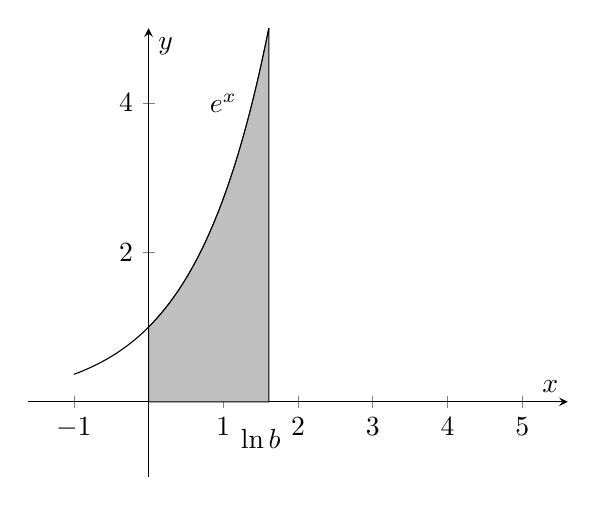
\begin{tikzpicture}
                        \begin{axis}[axis lines = middle,
                            domain  = -1:4,
                            xlabel  = {$x$},
                            ylabel  = {$y$},
                            axis equal,
                            xmin    = -1,
                            xmax    = 5,
                            ymin    = -1,
                            ymax    = 5,
                            samples = 300]
                            \addplot[thin] {e^x};
                            \draw[fill=gray!50] plot[domain=0:1.61] (\x, e^\x) |- (0,0) -- cycle;
                            \node at (1.5, -0.5) {$\ln b$};
                            \node at (1, 4) {$e^x$};
                        \end{axis}
                    \end{tikzpicture}
                \end{center}
                The area of the shaded region is $\int_0^{\ln b} e^x\,dx=e^x\Big|_0^{\ln b}=e^{\ln b}-e^0=b-1$.

                Below, I draw the diagram for (ii). Notice that reflecting the graph of $e^x$ across the line $y=x$ produces the graph of $\ln(x)$.
                \begin{center}
                    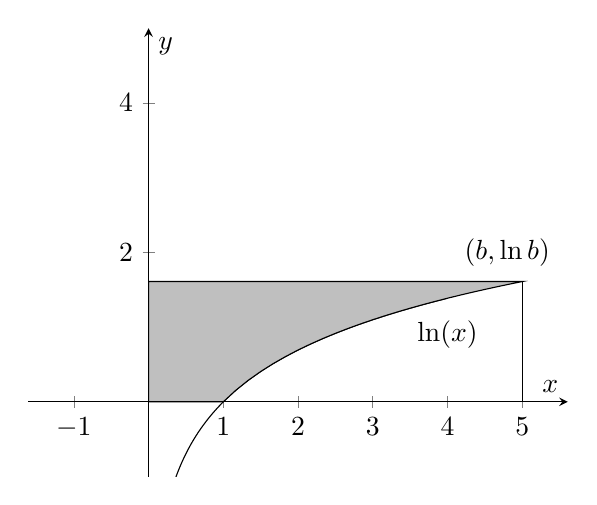
\begin{tikzpicture}
                        \begin{axis}[axis lines = middle,
                            domain  = -1:4,
                            xlabel  = {$x$},
                            ylabel  = {$y$},
                            axis equal,
                            xmin    = -1,
                            xmax    = 5,
                            ymin    = -1,
                            ymax    = 5,
                            samples = 300]
                        \addplot[thin] {ln(x)};
                        \draw[fill=gray!50] plot[domain=1:e^1.61] (\x,ln \x) -| (0,0) -- cycle;
                        \draw (0,0) -- (e^1.61, 0) -- (e^1.61, 1.61) -- (0, 1.61) -- cycle;
                        \node at (4, 0.9) {$\ln(x)$};
                        \node at (4.8, 2) {$(b, \ln b)$};
                        \end{axis}
                    \end{tikzpicture}
                \end{center}
                Now we answer (iii). The area of the shaded region in the second diagram is still $b-1$ because all we did to it was a reflection. The area of the rectangle is $b\cdot\ln b$. Therefore the unshaded region within the rectangle has area $b\ln b-(b-1)=b\ln b-b+1$. We can also see that the area of the unshaded part of the rectangle can be seen as the area under the graph of $\ln(x)$ from 1 to $b$, which is represented by the definite integral $\int_1^b \ln(x)\,dx$. Putting everything together we get
                \[\int_1^b\ln(x)\,dx=b\ln b-b+1,\]
                as desired.
            \end{solution}
        \end{enumerate}
    \end{problem}

\end{document}
